\section{Τι είναι παράλληλος προγραμματισμός}

\en{\url{https://hpc.llnl.gov/documentation/tutorials/introduction-parallel-computing-tutorial}}

Παραδοσιακά, τα προγράμματα γράφονται για σειριακή εκτέλεση και υπολογισμούς. Ένα πρόβλημα αναλύεται σε μία σειρά διακριτών εντολών οι οποίες εκτελούνται διαδοχικά η μία μετά την άλλη από έναν μόνο επεξεργαστή. Μόνο μία εντολή μπορεί να εκτελεστεί ανά πάσα στιγμή.

\begin{figure}[h!]
    \centering
    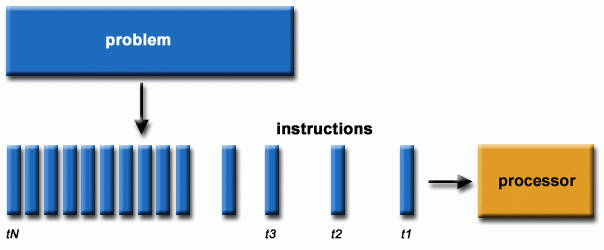
\includegraphics[scale=0.45]{images/Ch3/serial-execution.png}
    \caption{Παράδειγμα σειριακής υπολογιστικής}
    \label{fig:serial problem}
\end{figure}

Ο παράλληλος προγραμματισμός αναφέρεται στην ταυτόχρονη χρήση πολλαπλών υπολογιστικών πόρων για την επίλυση ενός υπολογιστικού προβλήματος. Το πρόβλημα χωρίζεται σε διακριτά μέρη που μπορούν να επιλυθούν ταυτόχρονα. Κάθε μέρος αναλύεται περαιτέρω σε μια σειρά εντολών , οι οποίες εκτελούνται ταυτόχρονα σε διαφορετικούς επεξεργαστές.  Επιπλέον, υπάρχει ένας κεντρικός μηχανισμός που συντονίζει και ελέγχει την εκτέλεση όλων αυτών.\cite{llnl}

\begin{figure}[h!]
    \centering
    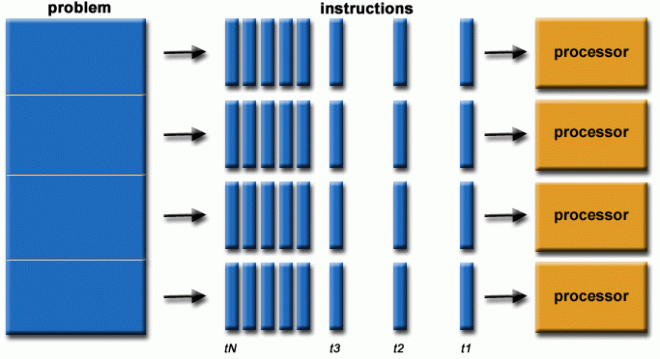
\includegraphics[scale=0.4]{images/Ch3/parallel-execution.png}
    \caption{Παράδειγμα παράλληλης υπολογιστικής}
    \label{fig:parallel problem}
\end{figure}

\subsubsection{Γιατί Παράλληλος Προγραμματισμός;}

Στο σημερινό κόσμο, στον τομέα της επιστήμης και της τεχνολογίας,  ο όγκος των δεδομένων που χρειάζεται να επεξεργαστούμε αυξάνεται εκθετικά. Οι απαιτήσεις των εφαρμογών που δίνουν λύση σε πολλά σύγχρονα προβλήματα  επιβάλουν όλο και καλύτερες επιδόσεις στους επεξεργαστές. Ειδικότερα στον τομέα της τεχνητής νοημοσύνης και της μηχανικής μάθησης.

\begin{figure}[h!]
    \centering
    \begin{subfigure}[b]{0.48\textwidth}
        \centering
        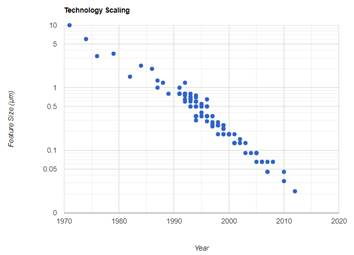
\includegraphics[width=\textwidth]{images/Ch3/technology-scaling.jpg}
        % \caption{\en{Technology Scaling}}
        % \label{fig:technology scaling}
    \end{subfigure}
    \hfill
    \begin{subfigure}[b]{0.48\textwidth}
        \centering
        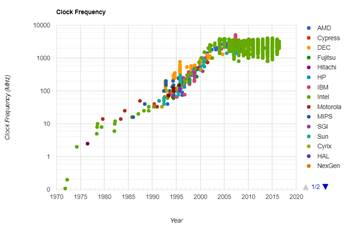
\includegraphics[width=\textwidth]{images/Ch3/clock-frequency.jpg}
        % \caption{\en{Clock Frequency}}
        % \label{fig:clock frequency}
    \end{subfigure}
    \caption{\en{Transistor Scaling and Clock Frequency}\cite{cpudb}}
    \label{fig:scaling-clock}
\end{figure}
 
Η αύξηση της απόδοσης των σειριακών επεξεργαστών έχει σταματήσει, καθώς οι σχεδιαστές επεξεργαστών έχουν φθάσει στα όρια της σμίκρυνσης, της συχνότητας ρολογιού, της ισχύος, ακόμη και της θερμότητας. 
Με την πάροδο του χρόνου, το μέγεθος των τρανζίστορ έχει μειωθεί. Λειτουργούν ταχύτερα, καταναλώνουν λιγότερη ενέργεια και μπορούμε να τοποθετήσουμε περισσότερα σε ένα ολοκληρωμένο κύκλωμα. 
Η αύξηση της συχνότητας του ρολογιού σε έναν επεξεργαστή, έχει σταματήσει λόγο της μεγάλης κατανάλωσης ενέργειας και την έκλυση θερμότητας που αυτή συνεπάγεται.
	
Καθώς η κατανάλωση ισχύος είναι από τους πιο σημαντικούς παράγοντες στον σχεδιασμό σύγχρονων επεξεργαστών, η αύξηση της υπολογιστικής ισχύος, σήμερα, επιτυγχάνεται κυρίως μέσω της προσθήκης όλο και περισσότερων υπολογιστικών πυρήνων στους επεξεργαστές. Αυτή η τάση της αύξησης του αριθμού των πυρήνων αντί της ταχύτητας του ρολογιού φαίνεται να επιτυγχάνει την ιδανικότερη απόδοση από άποψη κατανάλωσης αλλά και επεξεργαστικής ισχύος. 
Για να μπορέσουμε να αξιοποιήσουμε αυτού του είδους του \en{hardware} πρέπει να ξεφύγουμε από τον σειριακό τρόπο σκέψης στον προγραμματισμό και να αρχίσουμε να σκεφτόμαστε παράλληλα.

% \begin{figure}
%     \centering
%     \begin{subfigure}[b]{0.3\textwidth}
%         \centering
%         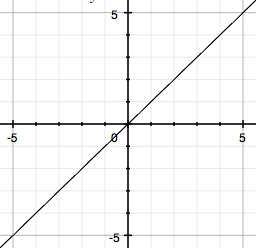
\includegraphics[width=\textwidth]{graph1}
%         \caption{$y=x$}
%         \label{fig:y equals x}
%     \end{subfigure}
%     \hfill
%     \begin{subfigure}[b]{0.3\textwidth}
%         \centering
%         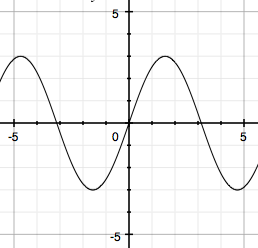
\includegraphics[width=\textwidth]{graph2}
%         \caption{$y=3sinx$}
%         \label{fig:three sin x}
%     \end{subfigure}
%     \hfill
%     \begin{subfigure}[b]{0.3\textwidth}
%         \centering
%         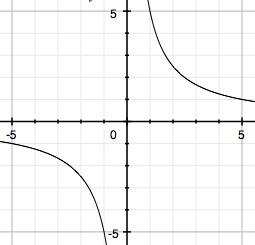
\includegraphics[width=\textwidth]{graph3}
%         \caption{$y=5/x$}
%         \label{fig:five over x}
%     \end{subfigure}
%     \caption{Three simple graphs}
%     \label{fig:three graphs}
% \end{figure}


